\documentclass[11pt]{article}
\usepackage[a4paper,margin=2.3cm]{geometry}
\usepackage[T1]{fontenc}
\usepackage[utf8]{inputenc}
\usepackage{mathptmx}
\usepackage{microtype}
\usepackage{amsmath,amssymb}
\usepackage{booktabs}
\usepackage{array}
\newcolumntype{L}[1]{>{\raggedright\arraybackslash}p{#1}}
\usepackage{graphicx}
\usepackage{caption}
\usepackage{xcolor}
\usepackage[numbers,sort&compress]{natbib}
\usepackage[colorlinks=true,linkcolor=blue!50!black,citecolor=blue!50!black,urlcolor=blue!50!black]{hyperref}
\captionsetup{font=small,labelfont=bf}
\setlength{\tabcolsep}{4pt}
\newcommand{\Hz}{\,Hz}

\title{History, Adaptation and a Missing Gain Estimate:\\ Two Pre-registered Tests of Learned Predictive Control\\ in a Synthetic Neural Population}
\author{Mahesh Reddy Pagadala\\ \small Aston University, Birmingham, UK}
\date{October 2026}

\begin{document}
\maketitle

\begin{abstract}
We study learned one-step predictive control of a synthetic population of 64 leaky integrate-and-fire neurons whose light sensitivity is scaled by a hidden factor $s$, using two pre-registered confirmations on plants simulated only after the analysis was frozen. In the first (50 plants, 11 conditions), a 200-ms input--output history was necessary for a parameter-matched neural predictor (removing it raised tracking RMSE by <<p1a_abs>>\Hz{} at $s=0.6$, 97.5\% CI <<p1a_lo>>--<<p1a_hi>>); a fixed linear model with the same history was practically equivalent at low gain; in secondary and benchmark comparisons, recursively adapted ARX had the lowest error in 10 of 11 conditions, development-tuned PI with anti-windup matched or beat the neural predictor for $s\ge0.7$, and training the predictor for 10\,000 rather than 900 epochs lowered prediction error but worsened control. Development work then pointed to one cause: the network does not infer the plant gain from its history. A second protocol (50 new plants, 9 sensitivities, 2 noise levels) confirmed three pre-specified predictions at the primary noise level. Re-estimating a single multiplicative input gain recovered <<q1pct>>\% (95\% CI <<q1pct_lo>>--<<q1pct_hi>>\%) of the benefit of full adaptive ARX. Giving the network that online gain estimate as an extra input reduced high-gain tracking error by <<q3>>\Hz{} <<q3ci>>. Longer training worsened the plain network by <<q4plain_abs>>\Hz{} but improved the gain-input network by <<q4gain_abs>>\Hz{}, a differential of <<q4>>\Hz{} <<q4ci>>. In secondary comparisons, the gain-input network came within 0.06\Hz{} of adaptive ARX and beat anti-windup PI at every sensitivity. Under high process noise the effects shrank to about 0.04\Hz{} or less and gain-only adaptation recovered only <<rq1pct>>\% of the adaptive-ARX benefit. In this synthetic system, explicit online estimation of one hidden parameter---an established idea in learning-based control---accounts for most of the gap between a history-based neural predictor and adaptive linear control, and for the mismatch between its prediction and control performance.
\end{abstract}

\section{Introduction}
Closed-loop control of neural population firing rates is used to probe circuit dynamics and is a component of proposed neural-interface systems. In optogenetic settings the effective plant gain can vary with opsin expression, optical attenuation and excitability, while the controller observes only the rate it produces~\cite{newman2015}. Learned dynamics models combined with sampling-based action selection are an attractive way to handle such systems~\cite{nagabandi2018}, but whether their extra capacity helps, and whether improving their predictive accuracy improves control, are empirical questions. We study them in a synthetic plant only and make no biological claim.

The work proceeded in two stages, each ending in a frozen protocol and a single run on untouched plants. The first stage asked: (i) does a learned one-step predictor need temporal input--output history once training data and capacity are matched; (ii) does a linear predictor with the same information suffice; (iii) how do learned and linear predictors compare with properly tuned PI and with online linear adaptation; and (iv) does a more accurate one-step predictor yield a better controller? Its answers raised a further question: (v) \emph{why} does online linear adaptation beat the learned predictor, and why does longer training make the learned predictor a worse controller? The second stage tested one mechanistic explanation for both: the hidden shift is a single multiplicative input gain, adaptive ARX succeeds by re-estimating it, and the network fails because it does not recover it from its history window.

\paragraph{Contributions.}
(1)~A matched history ablation, an aligned-pair chronology perturbation and a practical-equivalence test of linear sufficiency. (2)~A regime-stratified comparison against PI tuned on development plants, with and without anti-windup, and against recursively adapted ARX. (3)~A pre-specified secondary comparison showing prediction--control mismatch arising from training length, an instance of objective mismatch~\cite{lambert2020}, later tested as a primary hypothesis. (4)~A prospective test showing that a one-parameter gain estimate accounts for most of the adaptive-ARX advantage, and that supplying it to the network removes both the high-gain failure and the training-length mismatch. (5)~A documented methodological history (Appendix~\ref{app:history}): an earlier phase used an under-tuned PI and an RLS whose updates were negligible; both were corrected on development plants before any fresh confirmation.

\section{Related work}
\paragraph{Closed-loop optogenetic and neural control.} PI-type optogenetic feedback control of population activity has been demonstrated experimentally~\cite{newman2015}; the light required varied widely across preparations, which motivates treating plant gain as unknown. Model-based designs using identified input--output models have been developed for in-vivo use~\cite{bolus2018,grosenick2015}, including LQR control with a parameter-adaptive Kalman filter that tracks a drifting disturbance; re-estimating the input matrix was suggested as future work~\cite{bolus2021}. Learned forecasting models with model predictive control have been applied to a conductance-based neuron model, where a simple proportional controller was sometimes better~\cite{fehrman2023}, and to spiking networks via latent manifolds, where MPC outperformed PID~\cite{fehrman2024}. None of these compares a history-conditioned learned predictor with adaptive linear and tuned PI controllers under hidden gain shifts.

\paragraph{Identification, adaptation and history.} ARX models with recursive least squares and certainty-equivalence adaptive control are classical tools~\cite{astrom1995adaptive,ljung1999}; PI tuning and integrator anti-windup are covered in~\cite{astrom1995pid}. In learning-based control, recent input--output history is used to infer hidden parameters implicitly~\cite{kumar2021rma} or explicitly, by feeding an online system-identification estimate to a universal policy~\cite{yu2017}, typically under domain randomisation~\cite{tobin2017}. Our gain-input intervention is an instance of the explicit approach; it is not a new method.

\paragraph{Learned dynamics, fair baselines and objective mismatch.} That one-step model accuracy and control performance can diverge was shown in model-based reinforcement learning~\cite{lambert2020} and argued through value equivalence~\cite{grimm2020}. Equalising information and tuning between learned and classical controllers can shrink reported gaps~\cite{kunapuli2025}, although in-context learned models have outperformed PI on nonlinear motor loads~\cite{jian2026}.

\paragraph{Novelty boundary.} None of these methods or phenomena is new; we do not claim to have discovered objective mismatch or explicit parameter estimation. To our knowledge, the contribution is their combination in neural-population rate control: pre-registered, prospectively confirmed comparisons under hidden gain shifts, and a prospective test that a one-parameter gain estimate explains both the advantage of adaptive linear control and the prediction--control mismatch of the learned predictor in this setting.

\section{Methods}
\subsection{Plant}
The plant is a population of $N=64$ leaky integrate-and-fire-like neurons sharing a scalar light command $u\in[0,1]$. Each neuron has initial potential $V_i(0)\sim U(-65,-55)$, bias $b_i\sim U(7,12)$ and light sensitivity $\kappa_i\sim U(18,26)$, drawn from a generator seeded by the plant seed (model voltage units). Each 50-ms control step is integrated with 50 Euler sub-steps of 1\,ms. A phenomenological first-order gate (time constant 10\,ms) filters the command, $g\leftarrow g+(u-g)/10$, and each non-refractory neuron updates as
\begin{equation}
V_i \leftarrow V_i + \tfrac{1}{20}\big[-(V_i+65) + b_i + s\,\kappa_i\, g\big] + \sigma\xi,\qquad \xi\sim\mathcal N(0,1).
\end{equation}
A neuron reaching $-50$ spikes, resets to $-65$ and is refractory for 2\,ms. The observed output is the smoothed population rate $y_t=0.5\,y_{t-1}+0.5\,r_t$ (Hz per neuron). The hidden multiplier $s$ scales every $\kappa_i$; $\sigma$ is per-sub-step process noise. No controller receives $s$ or $\sigma$. Each episode lasts 180 steps (9\,s) and tracks 12, 30, 20, 40, 15 and 35\Hz, each held for 30 steps. The gate is not an opsin kinetic model.

\subsection{Training data and predictors}
All learned and linear predictors were fitted to plants 2000--2099 (training) and 2100--2129 (validation), 300 steps each, with per-plant $\sigma\sim U(0.5,2)$, $s\sim U(0.6,1.4)$ and bias shift $\sim U(-2,2)$, and the light command resampled from $U(0,1)$ every four steps (open-loop excitation). Rates are scaled by $1/60$. Networks are $9\to64\to1$ tanh multilayer perceptrons (DR-H4) whose inputs are the four past rates, the four past actions and a candidate action, trained by full-batch Adam on squared one-step error (learning rate 0.006), five initialisations each, keeping the best-validation weights within the stated epoch budget. The memoryless control (Mem-141, $3\to141\to1$, 706 parameters, matched to DR-H4) sees only the current rate, the previous action and the candidate. The ARX prior is linear in the same ten regressors (candidate action, four rates, four past actions, constant), fitted by least squares on the training data.

\subsection{Controllers}
All predictive controllers apply the action minimising $(\hat y_{t+1}(u)-r_t)^2+2u^2+2(u-u_{t-1})^2$ over 101 candidates in $[0,1]$; this is one-step grid-search predictive control, not receding-horizon MPC or reinforcement learning. Table~\ref{tab:arms} lists the arms of both protocols.

\begin{table}[t]\centering\small
\caption{Controllers. Network arms have five initialisations each, averaged within plant. Every gain, epoch and checkpoint was fixed on training, validation or development plants before the corresponding confirmation.}\label{tab:arms}
\begin{tabular}{@{}L{3.1cm}L{9.6cm}L{1.6cm}@{}}\toprule
Arm & Definition & Protocol\\\midrule
PI tuned & positional PI, $K_p=0.02$, $K_i=0.20$, integrator clip $\pm10$ (development grid of 400 gain pairs) & v3, v4\\
PI tuned + AW & as above with back-calculation anti-windup, $K_p=0.02$, $K_i=0.25$, $k_t=0.5$ & v3, v4\\
PI sens.\ ref. & best PI of the family when $s$ is known; not deployable, reference only & v3\\
ARX fixed & least-squares prior, no online update & v3, v4\\
ARX + RLS & all ten coefficients adapted by RLS, $P_0=10^9\hat\sigma^2(\Phi^\top\Phi)^+$, $\lambda=0.98$ & v3, v4\\
ARX-$g$ & one-parameter gain RLS (Section~\ref{sec:gain}), $P_0=1000$, $\lambda=0.98$ & v4\\
H4-10k & DR-H4, 10\,000-epoch budget, best validation & v3, v4\\
H4-900 & DR-H4, 900-epoch budget & v3, v4\\
Mem-141 & memoryless network, 10\,000-epoch budget & v3\\
I1 & DR-H4 raw snapshot at a per-seed epoch (300--900) chosen by closed-loop error on development plants 5250--5299 & v4\\
I2 & DR-H4 with the online gain estimate $g$ as a tenth input; best validation within 6000 epochs & v4\\
I3 & DR-H4 retrained on open-loop data plus closed-loop trajectories of its own 10k model; best validation within 6000 epochs & v4\\
H4 / I2 at epoch 900, 6000 & raw weights at fixed epochs from checkpointed retraining (for the matched-epoch test) & v4\\\bottomrule
\end{tabular}\end{table}

\subsection{One-parameter gain estimator}\label{sec:gain}
Split the ARX prior $w_0$ into action terms $a_t=z_t^\top w_a$ (candidate and four past actions) and the rest $z_t^\top w_r$. The gain estimator predicts $\hat y_{t+1}=z_t^\top w_r + g\,a_t$ and updates the scalar $g$ by RLS with forgetting factor 0.98, $P_0=1000$ and $g_0=1$ after every step. ARX-$g$ uses this predictor for control. In I2 the same estimator runs alongside the network, and its current $g$ is the network's tenth input; for training, $g$ was computed on the open-loop training trajectories before each next rate was observed. The estimator, its settings and its use are identical at both noise levels.

\subsection{Interventions and checkpoints}
Three interventions were developed on plants 5200--5299 to address the training-length mismatch: I1 (closed-loop early stopping), I2 (gain input) and I3 (on-policy data; closed-loop trajectories at random targets of 10--45\Hz{} held for 30 steps). For the matched-epoch test the plain DR-H4 was retrained with weights saved at fixed epochs; its epoch-900 weights reproduce the original 900-epoch weights to within $10^{-15}$. No checkpoint, epoch, model variant or estimator setting was chosen on confirmation plants.

\subsection{Study design}
Each protocol was frozen before its confirmation plants were instantiated, with SHA-256 hashes of the script, protocol, simulator modules, ARX prior and every weight file recorded in a manifest that the run script re-checks on every invocation. Each confirmation block was simulated once with the exact scalar simulator. Confirmation blocks were never reused, and no development block overlaps a confirmation block (Appendix~\ref{app:history}).

\textbf{Protocol v3} (plants 7000--7049): $s\in\{0.5,0.6,\dots,1.2,1.4\}$ at $\sigma=0.5$ ($s=0.5$ lies outside the training range), plus $\sigma\in\{1,2\}$ at $s=1$. \textbf{Protocol v4} (plants 8000--8049): the same nine sensitivities at $\sigma=0.5$ (primary) and $\sigma=2.0$ (robustness), 900 plant-conditions.

\subsection{Hypotheses and statistics}
The unit of analysis is the plant: network RMSE (180 steps) is averaged over the five initialisations within each plant before paired differences are formed. Intervals are bias-corrected and accelerated (BCa) bootstrap intervals~\cite{efron1987} with 10\,000 resamples and a fixed bootstrap seed per interval, Bonferroni-corrected within each family. Table~\ref{tab:hyp} lists all pre-specified tests. In v4, the high-gain set $\mathcal H=\{1.0,1.1,1.2,1.4\}$ was fixed in advance, and Q1 is the ratio of plant-level means
\begin{equation}
Q_1=\frac{\overline{\textstyle\frac19\sum_s(\mathrm{ARX}_{\mathrm{fixed}}-\mathrm{ARX}_g)}}{\overline{\textstyle\frac19\sum_s(\mathrm{ARX}_{\mathrm{fixed}}-\mathrm{ARX}_{\mathrm{RLS}})}},
\end{equation}
with the bar denoting the mean over plants. Q4 is a difference-in-differences at matched epochs, $D=[\text{H4}_{6000}-\text{H4}_{900}]-[\text{I2}_{6000}-\text{I2}_{900}]$, averaged over $\mathcal H$. A positive $D$ supports a differential effect only; the directions of the two components were tested separately. A former hypothesis Q2 (monotonicity of $g$ in $s$) was moved to secondary before the freeze, hence the gap in numbering.

\begin{table}[t]\centering\small
\caption{Pre-specified tests. Secondary results do not change primary decisions. Development values for v4 came from plants 5200--5249.}\label{tab:hyp}
\begin{tabular}{@{}llL{7.6cm}L{4.4cm}@{}}\toprule
Protocol & ID & Contrast & Level / decision\\\midrule
v3 & P1 & Mem-141 $-$ H4-10k at $s=0.6, 0.8$ & 97.5\% each; both lower bounds $>0$\\
v3 & P2 & ARX fixed $-$ H4-10k at $s=0.6$ & 95\%; interval within $\pm0.25$\Hz\\
v3 & B1 & PI tuned (+AW) $-$ H4-10k, 11 conditions & 99.77\% each; no direction\\
v3 & S1, S3--S5 & RLS effect, chronology shuffle, ARX+RLS $-$ H4-10k, H4-900 $-$ H4-10k & 97.5--99.55\%; exploratory\\
v4 & Q1 & gain fraction, $\sigma=0.5$ & 95\%; lower bound $\ge0.70$\\
v4 & Q3 & H4-10k $-$ I2, mean over $\mathcal H$, $\sigma=0.5$ & 95\%; lower bound $>0$\\
v4 & Q4 & $D$ over $\mathcal H$, $\sigma=0.5$ & 95\%; lower bound $>0$\\
v4 & secondary & directions of Q4 components; Spearman$(g,s)$ per plant; calibration of $g$; Q3 per setting; I2 $-$ ARX+RLS (no equivalence claim); I1, I3 vs H4-10k; I2 $-$ PI+AW; action-sensitivity slope & 97.5--99.44\%\\
v4 & R & Q1, Q3, Q4 at $\sigma=2.0$ & 98.3\% each; robustness\\\bottomrule
\end{tabular}\end{table}

\section{Results: protocol v3}
Both primary hypotheses were supported. Table~\ref{tab:v3} and Figure~\ref{fig:v3} give mean tracking RMSE for every controller and condition.

\begin{table}[t]\centering\small
\caption{Protocol v3: mean tracking RMSE (Hz) over 50 confirmation plants (7000--7049). Lowest of the deployable arms shown in bold. $^\dagger$Uses knowledge of $s$; excluded from bold. A legacy PI with phase-1 gains ($K_i=0.15$, not shown) was 0.004\Hz{} lower than ARX+RLS at $s=1.4$ and higher elsewhere.}\label{tab:v3}
\begin{tabular}{@{}lrrrrrrrr@{}}\toprule
<<table_v3_head>>\midrule
<<table_v3>>
\bottomrule\end{tabular}\end{table}

\begin{figure}[t]\centering
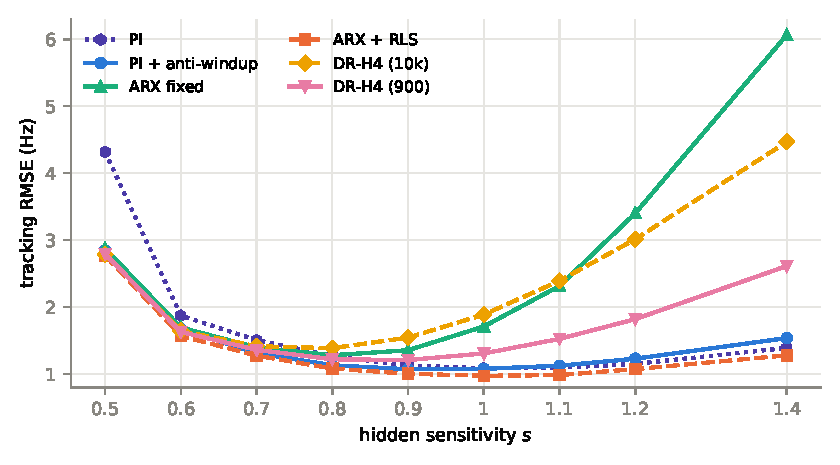
\includegraphics[width=0.78\linewidth]{fig1_v3_rmse.pdf}
\caption{Protocol v3: mean tracking RMSE against hidden sensitivity at $\sigma=0.5$. The memoryless network (1.7--5.6\Hz) is omitted for scale; all values are in Table~\ref{tab:v3}.}\label{fig:v3}
\end{figure}

\paragraph{History is necessary (P1).} With training data and parameter count matched, removing the history increased RMSE by <<p1a>>\Hz{} at $s=0.6$ and <<p1b>>\Hz{} at $s=0.8$ (97.5\% intervals), on every plant. In a secondary test (S3), a joint permutation of the history raised RMSE by <<s3a>> and <<s3b>>\Hz{}. Because permuted histories never occur in training, this shows that the controller depends on temporal order, not that it estimates the plant gain. P1 was tested only at $s=0.6$ and $0.8$; at $s\ge1.0$ the memoryless network tracked better than H4-10k (Table~\ref{tab:v3}), consistent with the 10k network's high-gain failure examined in Section~6.

\paragraph{A linear model with the same history suffices at low gain (P2).} At $s=0.6$ the fixed ARX differed from H4-10k by <<p2>>\Hz{} (95\%), within the $\pm0.25$-Hz margin. Away from low gain the fixed ARX degrades sharply (<<arxf12>>\Hz{} at $s=1.2$, <<arxf14>>\Hz{} at 1.4).

\paragraph{Tuned PI matches or beats the learned predictor from $s=0.7$ (B1).} The network kept an advantage only where PI was saturated or noise-limited: at $s\le0.6$, and at $\sigma=2$, where the zero-light rate floor exceeds the 12-Hz target (anti-windup PI <<awn2>>\Hz). Against anti-windup PI the low-gain advantage was small (<<aw06>>\Hz{} at $s=0.6$). From $s=0.7$ upwards anti-windup PI was better on every plant, by <<aw07>>\Hz{} at 0.7 rising to <<aw14>>\Hz{} at 1.4 (Table~\ref{tab:b1}).

\paragraph{Online linear adaptation is the strongest controller (S1, S4).} RLS improved the fixed ARX in every condition, by <<s1_lo>>\Hz{} at $\sigma=2$ to <<s1_hi>>\Hz{} at $s=1.4$. Adaptive ARX beat H4-10k in <<s4n>> of 11 conditions and was indistinguishable from it in the other two; it had the lowest mean RMSE among deployable controllers in ten of eleven conditions (at $s=1.4$ the legacy PI was <<rls14_vs_legacy>>\Hz{} lower) and came within 0.03\Hz{} of the sensitivity-informed PI reference at $s=1.2$ (<<rls12>> vs <<ref12>>\Hz).

\paragraph{Better prediction, worse control (S5, secondary).} The 10k models had lower one-step validation RMSE than the 900-epoch models (1.39--1.40 vs 1.61--1.85\Hz) but tracked worse at every $s\ge0.6$ and at $\sigma=1$ (by only 0.015\Hz{} at $s=0.6$): by <<s5_07>>\Hz{} at $s=0.7$, <<s5_10>>\Hz{} at 1.0 and <<s5_14>>\Hz{} at 1.4. This comparison was added after a development observation and was secondary.

\begin{table}[t]\centering\small
\caption{Protocol v3: PI minus H4-10k RMSE (Hz) with simultaneous 95\% intervals (99.77\% each). Negative values favour PI.}\label{tab:b1}
\begin{tabular}{@{}lll@{}}\toprule
Condition & PI tuned $-$ H4-10k & PI + AW $-$ H4-10k\\\midrule
<<table_b1>>
\bottomrule\end{tabular}\end{table}

\section{From v3 to v4: development findings}
On fresh development plants (5200--5249 for evaluation; 5250--5299 only for selecting I1's epochs), three observations motivated the second protocol. (a)~In the full RLS, the coefficient on the candidate action tracked $s$ almost perfectly, but adapting that coefficient alone recovered little, because the gain also enters through the four lagged-action terms. One scalar multiplying all five action terms tracked $s$ linearly and recovered 86\% of the full-RLS benefit. (b)~Across 60 training checkpoints, the correlation between open-loop validation error and closed-loop error fell from 0.81 at $s=0.6$ to $-0.08$ at $s=1.4$; the network's local action sensitivity $\partial\hat y/\partial u$ stayed nearly constant across $s$ instead of scaling with the plant gain. (c)~Of three interventions, supplying the gain estimate as an input (I2) brought the network's mean RMSE from 2.29 to 1.35\Hz, close to full adaptive ARX (1.33\Hz), and made longer training help instead of hurt. All three findings were then frozen as v4 hypotheses (Table~\ref{tab:hyp}).

\section{Results: protocol v4}
All three primary hypotheses were supported (Table~\ref{tab:primary}). Mean RMSE for every arm is in Table~\ref{tab:v4} and Figure~\ref{fig:v4}.

\begin{table}[t]\centering\small
\caption{Protocol v4 primary decisions at $\sigma=0.5$ (plants 8000--8049; 95\% BCa intervals) and the same statistics at $\sigma=2.0$ (98.3\% intervals; robustness, not decisions). $^*$Development values at $s=1.0$ and $1.4$; no high-gain-set mean was recorded.}\label{tab:primary}
\begin{tabular}{@{}llllll@{}}\toprule
ID & Criterion & Development & $\sigma=0.5$ & Decision & $\sigma=2.0$\\\midrule
Q1 & lower bound $\ge0.70$ & 0.86 & <<q1>> <<q1ci>> & supported & <<rq1>> <<rq1ci>>\\
Q3 & lower bound $>0$ & +1.84\Hz & +<<q3>> <<q3ci>> & supported & +<<rq3>> <<rq3ci>>\\
Q4 & lower bound $>0$ & +1.0 to +3.8\Hz$^*$ & +<<q4>> <<q4ci>> & supported & +<<rq4>> <<rq4ci>>\\\bottomrule
\end{tabular}\end{table}

\begin{table}[t]\centering\small
\caption{Protocol v4: mean tracking RMSE (Hz) over 50 plants. ARX-$g$: one-parameter gain RLS; I1--I3: interventions. Lowest in each row in bold. H4 and I2 at fixed epochs are in Figure~\ref{fig:train}.}\label{tab:v4}
\begin{tabular}{@{}lrrrrrrrrr@{}}\toprule
\multicolumn{10}{@{}l}{\emph{$\sigma=0.5$ (primary)}}\\
<<t4_head>>\midrule
<<t4a>>
\midrule
\multicolumn{10}{@{}l}{\emph{$\sigma=2.0$ (robustness)}}\\
<<t4_head>>\midrule
<<t4b>>
\bottomrule\end{tabular}\end{table}

\begin{figure}[t]\centering
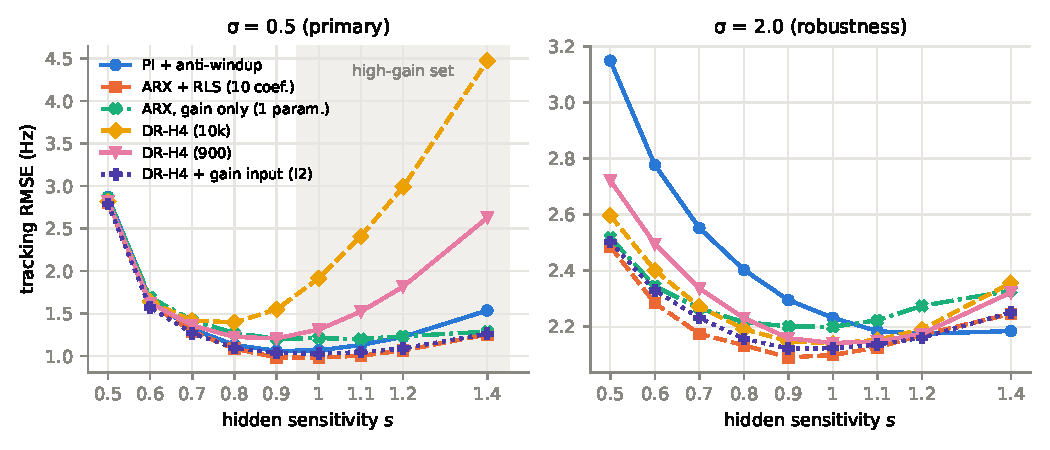
\includegraphics[width=\linewidth]{fig2_v4_rmse.pdf}
\caption{Protocol v4: mean tracking RMSE against hidden sensitivity for six arms. Shading marks the pre-specified high-gain set. All arms are in Table~\ref{tab:v4}.}\label{fig:v4}
\end{figure}

\subsection{One input gain accounts for most of the adaptive-ARX advantage (Q1)}
Adapting the single scalar $g$ recovered <<q1>> <<q1ci>> of the improvement that full ten-coefficient RLS achieves over the fixed ARX, above the 0.70 threshold. In secondary analyses, the estimate behaved as a gain estimate should (Figure~\ref{fig:g}): its rank correlation with $s$ was 1.0 on every one of the 50 plants (minimum <<q2_min>>); a per-plant linear fit gave slope <<cal_slope>> <<cal_slope_ci>> (99\%), intercept <<cal_int>> and mean absolute residual <<cal_res>>; the coefficient of variation of $g/s$ was <<cal_cv>>. Because $g$ multiplies the domain-randomised prior's action terms, its absolute scale is relative to that prior ($g=1$ at $s=1$ would mean no correction; observed $g-1=$ <<cal_g1>>).

\begin{figure}[t]\centering
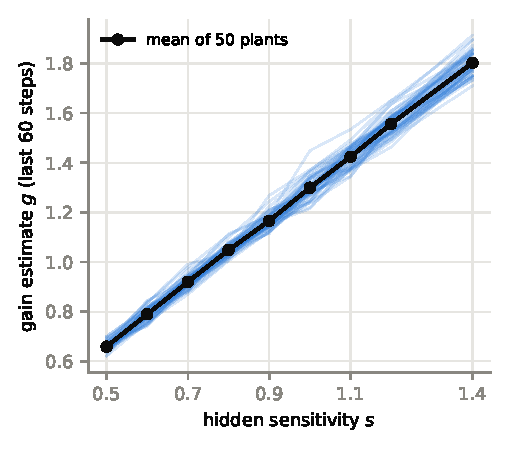
\includegraphics[width=0.45\linewidth]{fig4_gain_estimate.pdf}
\caption{Gain estimate $g$ (mean of the last 60 steps of ARX-$g$) against $s$ for each of the 50 v4 plants (thin lines) and their mean, $\sigma=0.5$.}\label{fig:g}
\end{figure}

\subsection{Supplying the gain estimate removes the high-gain failure (Q3)}
Over the high-gain set, I2 tracked better than H4-10k by <<q3>>\Hz{} <<q3ci>>. The advantage held at every high-gain setting and on every plant (Table~\ref{tab:q3}). Across all nine sensitivities I2 had a mean RMSE of <<m_i2>>\Hz, against <<m_10k>>\Hz{} for H4-10k and <<m_rls>>\Hz{} for full adaptive ARX. In a secondary analysis, the learned action sensitivity now scaled with the plant gain: the slope of $\partial\hat y/\partial u$ against $s$, relative to the slope of the gain-RLS reference, was <<slI2>> <<slI2ci>> for I2 versus <<sl10k>> <<sl10kci>> for H4-10k and <<sl900>> <<sl900ci>> for H4-900. The reference is itself the one-parameter estimate, not the plant's true local gain.

\begin{table}[t]\centering\small
\caption{H4-10k $-$ I2 at each high-gain setting ($\sigma=0.5$; 98.75\% intervals) and the share of plants with a positive difference.}\label{tab:q3}
\begin{tabular}{@{}lll@{}}\toprule
$s$ & H4-10k $-$ I2 (Hz) & plants $>0$\\\midrule
<<t_q3>>
\bottomrule\end{tabular}\end{table}

\subsection{The training-length mismatch is specific to the network without the gain (Q4)}
At matched epochs over the high-gain set, training from 900 to 6000 epochs changed the plain network's RMSE by <<q4plain>>\Hz{} and the gain-input network's by <<q4gain>>\Hz{} (97.5\% intervals). The directions are opposite, as pre-specified, and the difference-in-differences was <<q4>>\Hz{} <<q4ci>> (Figure~\ref{fig:train}). Given the gain estimate, more training improves both prediction and control; without it, more training improves prediction and degrades control.

\begin{figure}[t]\centering
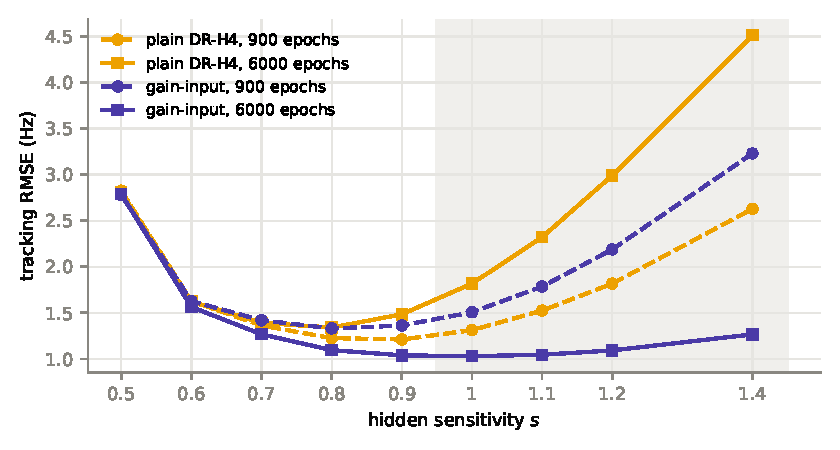
\includegraphics[width=0.78\linewidth]{fig3_training_length.pdf}
\caption{Matched-epoch comparison at $\sigma=0.5$: plain DR-H4 and gain-input I2 at 900 (dashed) and 6000 (solid) epochs. Shading marks the high-gain set.}\label{fig:train}
\end{figure}

\subsection{Secondary comparisons}
Table~\ref{tab:pairs} gives per-sensitivity paired contrasts. I2 and full adaptive ARX differed by between <<s1_min>> and <<s1_max>>\Hz{}: I2 was better at $s=$ <<s1_better>> and worse at $s=$ <<s1_worse>>, with no interval-excluding difference elsewhere. No equivalence margin was pre-specified, so we claim closeness, not equivalence. I2 beat anti-windup PI at <<s6_n>> of 9 sensitivities, by <<s6_lo>>--<<s6_hi>>\Hz. Closed-loop early stopping (I1) improved on H4-10k for $s\ge$ <<s2_pos_from>> and on-policy data (I3) at <<s3_pos_n>> of 9 sensitivities, but by much less than I2 at high gain (<<s2_14>> and <<s3_14>>\Hz{} at $s=1.4$, against <<sq3_hi>>\Hz{} for I2); I1 was slightly worse at $s=0.5$ (<<s2_05>>\Hz).

\begin{table}[t]\centering\footnotesize
\caption{Protocol v4 secondary contrasts at $\sigma=0.5$ (Hz; 99.44\% intervals). For I2 $-$ X, negative favours I2; for H4-10k $-$ X, positive favours X.}\label{tab:pairs}
\begin{tabular}{@{}lllll@{}}\toprule
$s$ & I2 $-$ ARX+RLS & I2 $-$ PI+AW & H4-10k $-$ I1 & H4-10k $-$ I3\\\midrule
<<t_pairs>>
\bottomrule\end{tabular}\end{table}

\subsection{Robustness at high process noise}
At $\sigma=2.0$, Q1 was <<rq1>> <<rq1ci>>: gain-only adaptation recovered only about a quarter of the full-RLS benefit, well below the threshold used at $\sigma=0.5$. Q3 and Q4 stayed positive but were small (<<rq3>> and <<rq4>>\Hz). At this noise level the predictive arms lay within about 0.15\Hz{} of each other on average (mean RMSE <<m_rls2>>\Hz{} for adaptive ARX, <<m_i22>> for I2, <<m_10k2>> for H4-10k), and anti-windup PI was worse (<<m_aw2>>\Hz). The mechanism we confirmed at $\sigma=0.5$ therefore matters little when process noise dominates the error.

\section{Discussion}
\paragraph{Information and adaptation, not nonlinear capacity.} History is indispensable for a learned predictor facing a hidden gain, but a linear model with the same history performs as well at low gain, and adapting that linear model online made it the best or near-best controller across almost the entire range in both protocols. Protocol v4 identifies what the adaptation provides: an estimate of one multiplicative input gain. A network trained across randomised gains, but never told the gain, learned an action sensitivity that changed far less than the plant gain did, so its errors grew steeply as the gain increased. Supplying the gain estimate fixed this, which is the explicit identification strategy of universal policies with online system identification~\cite{yu2017} applied to neural-population rate control.

\paragraph{Why better prediction gave worse control.} Without the gain, a network can lower average one-step error by fitting the open-loop data more closely while its action sensitivity remains wrong for any particular plant; the one-step controller then over- or under-acts. With the gain available, lower prediction error corresponds to a more accurate model of the current plant, and control improves. This account fits both confirmed results but rests on a single plant family and a single architecture; we offer it as an interpretation, consistent with objective mismatch in model-based reinforcement learning~\cite{lambert2020,grimm2020}, not as a general law.

\paragraph{Classical feedback is a hard baseline.} The apparent low-gain advantage of the learned controller in the earlier phase largely disappeared once PI was tuned on the same development data and given anti-windup. Claims that a learned controller beats classical control should state how the classical baseline was tuned~\cite{kunapuli2025}. Our results differ from the MPC-over-PID finding in spiking networks~\cite{fehrman2024}; candidate reasons are our one-step action selection, our tuned PI with anti-windup and our fully observed population rate. Among the learned predictors, only the gain-input network beat anti-windup PI at every sensitivity (full adaptive ARX also had lower mean RMSE than anti-windup PI at every sensitivity in v4).

\section{Limitations}
\begin{itemize}\setlength\itemsep{2pt}
\item \textbf{Synthetic plant.} Uncoupled LIF-like neurons with a phenomenological light gate; no recurrence, inhibition, plasticity, spatial light distribution or opsin kinetics. One plant family supplies training and test plants, and the shift is a scalar gain plus process noise, which suits a one-parameter estimator.
\item \textbf{Noise dependence.} The gain mechanism explains most of the effect at $\sigma=0.5$ but little at $\sigma=2.0$, where Q1 fell to <<rq1>>.
\item \textbf{Controller scope.} One-step action selection only; PI from one family tuned by grid search; one learned architecture. The action-sensitivity analysis uses the gain-RLS estimate as its reference, not the true local gain.
\item \textbf{Hypothesis origin.} All v4 hypotheses and the v3 training-length comparison were formed from development data; their confirmation on untouched plants is what we report.
\item \textbf{Run integrity.} Two v3 chunks ran concurrently by mistake and three v4 chunks were interrupted by infrastructure errors; affected plant-conditions were recomputed and matched exactly (Appendix~\ref{app:integrity}).
\end{itemize}

\section{Conclusion}
In a first pre-registered confirmation on untouched synthetic plants, short input--output history was necessary for a learned predictive controller under hidden gain shifts and a linear model with the same history was practically equivalent at low gain (primary hypotheses); in pre-specified secondary and benchmark comparisons, online linear adaptation outperformed it, anti-windup PI matched or beat it from moderate gain upwards, and longer training improved its predictions while worsening its control. A second protocol, with these observations turned into primary hypotheses, showed that most of this pattern follows from one missing quantity: re-estimating a single input gain recovered most of the benefit of adaptive ARX, and giving the network that estimate removed both its high-gain failure and its prediction--control mismatch at the primary noise level. For this class of problem, explicit estimation of the hidden parameter matters more than model expressiveness.

\section*{Code and data availability}
Code, frozen protocols (\texttt{PROTOCOL\_V3.json}, \texttt{PROTOCOL\_V4.json}), manifests, model weights, raw per-plant results, development records and the scripts that generate every number and figure in this paper: \url{https://github.com/lonewolf15116/NeuroLight-AI}.

\begin{thebibliography}{99}\small
\bibitem{newman2015} Newman JP, Fong M, Millard DC, Whitmire CJ, Stanley GB, Potter SM. Optogenetic feedback control of neural activity. \emph{eLife} 4:e07192, 2015. doi:10.7554/eLife.07192
\bibitem{nagabandi2018} Nagabandi A, Kahn G, Fearing RS, Levine S. Neural network dynamics for model-based deep reinforcement learning with model-free fine-tuning. \emph{IEEE International Conference on Robotics and Automation (ICRA)}, 2018. arXiv:1708.02596
\bibitem{lambert2020} Lambert N, Amos B, Yadan O, Calandra R. Objective mismatch in model-based reinforcement learning. \emph{Proc.\ 2nd Conference on Learning for Dynamics and Control}, PMLR 120:761--770, 2020. arXiv:2002.04523
\bibitem{bolus2018} Bolus MF, Willats AA, Whitmire CJ, Rozell CJ, Stanley GB. Design strategies for dynamic closed-loop optogenetic neurocontrol in vivo. \emph{Journal of Neural Engineering} 15(2):026011, 2018. doi:10.1088/1741-2552/aaa506
\bibitem{grosenick2015} Grosenick L, Marshel JH, Deisseroth K. Closed-loop and activity-guided optogenetic control. \emph{Neuron} 86(1):106--139, 2015. doi:10.1016/j.neuron.2015.03.034
\bibitem{bolus2021} Bolus MF, Willats AA, Rozell CJ, Stanley GB. State-space optimal feedback control of optogenetically driven neural activity. \emph{Journal of Neural Engineering} 18(3):036006, 2021. doi:10.1088/1741-2552/abb89c
\bibitem{fehrman2023} Fehrman C, Meliza CD. Nonlinear model predictive control of a conductance-based neuron model via data-driven forecasting. arXiv:2312.14274, 2023.
\bibitem{fehrman2024} Fehrman C, Meliza CD. Model predictive control on the neural manifold. arXiv:2406.14801, 2024.
\bibitem{astrom1995adaptive} {\AA}str{\"o}m KJ, Wittenmark B. \emph{Adaptive Control}, 2nd ed. Addison-Wesley, 1995. ISBN 0-201-55866-1
\bibitem{ljung1999} Ljung L. \emph{System Identification: Theory for the User}, 2nd ed. Prentice Hall PTR, Upper Saddle River, NJ, 1999.
\bibitem{astrom1995pid} {\AA}str{\"o}m KJ, H{\"a}gglund T. \emph{PID Controllers: Theory, Design, and Tuning}, 2nd ed. Instrument Society of America, Research Triangle Park, NC, 1995. ISBN 1-55617-516-7
\bibitem{kumar2021rma} Kumar A, Fu Z, Pathak D, Malik J. RMA: Rapid motor adaptation for legged robots. arXiv:2107.04034, 2021.
\bibitem{yu2017} Yu W, Tan J, Liu CK, Turk G. Preparing for the unknown: learning a universal policy with online system identification. arXiv:1702.02453, 2017.
\bibitem{tobin2017} Tobin J, Fong R, Ray A, Schneider J, Zaremba W, Abbeel P. Domain randomization for transferring deep neural networks from simulation to the real world. \emph{IEEE/RSJ IROS}, pp.\ 23--30, 2017. doi:10.1109/IROS.2017.8202133
\bibitem{grimm2020} Grimm C, Barreto A, Singh S, Silver D. The value equivalence principle for model-based reinforcement learning. arXiv:2011.03506, 2020.
\bibitem{kunapuli2025} Kunapuli P, Welde J, Jayaraman D, Kumar V. Leveling the playing field: carefully comparing classical and learned controllers for quadrotor trajectory tracking. arXiv:2506.17832, 2025.
\bibitem{jian2026} Jian T, Dai T, Yu T. Learning nonlinear systems in-context: from synthetic data to real-world motor control. arXiv:2602.07173, 2026.
\bibitem{efron1987} Efron B. Better bootstrap confidence intervals. \emph{Journal of the American Statistical Association} 82(397):171--185, 1987. doi:10.1080/01621459.1987.10478410
\end{thebibliography}

\appendix
\section{Study history}\label{app:history}
\begin{table}[h]\centering\small
\begin{tabular}{@{}llL{7.6cm}@{}}\toprule
Stage & Plants & Outcome\\\midrule
v0.1--v0.6 (exploratory) & 0--69, 1000--1049, 1400--1649 & learned controller brittle to gain shift; history helps\\
C0 confirmation & 3000--3049 & chronology effect +2.1 / +5.4\Hz\\
Experiment A & 4000--4049 & matched history ablation +2.76\Hz{} at $s=0.6$\\
Experiment B & 6000--6049 & linear equivalence at $s=0.6$; PI later found under-tuned, RLS inactive\\
Phase-2 development & 5000--5149 & PI search, adaptive RLS, 10\,000-epoch retraining, rehearsal\\
\textbf{v3 confirmation} & 7000--7049 & Section~4\\
Phase-4 development & 5200--5299 & gain mechanism, checkpoints, interventions (Section 5)\\
\textbf{v4 confirmation} & 8000--8049 & Section 6\\\bottomrule
\end{tabular}\end{table}
Phase-1 results are retained as historical records and are not pooled with v3 or v4. In phase 1, PI's integral gain lay on the edge of its tuning grid and switching RLS updates off changed RMSE by less than 0.01\Hz; both were corrected on development plants before v3.

\section{Run integrity}\label{app:integrity}
\textbf{v3.} The confirmation ran in nine resumable invocations on a laptop. Two were accidentally launched concurrently and wrote the same progress file. The simulator is deterministic per plant and each write is a complete snapshot, so the only possible effect is duplicated work; all 200 plant-conditions in the four affected conditions were recomputed from the frozen code, with a maximum absolute difference of 0.0.

\textbf{v4.} The confirmation ran in resumable chunks of at most 172\,s, one at a time. Three invocations returned infrastructure errors with unknown execution status (at about 465, 561 and 869 of 900 plant-conditions); each resume waited until the progress file had been unchanged for over three minutes. Ten plant-conditions---those on both sides of every interruption, plus the first and last primary plant---were recomputed from scratch in a separate environment; all 302 recorded values of each matched exactly. Recomputing every statistic from the stored raw data reproduced the reported values to $3\times10^{-16}$. Results file SHA-256: \texttt{\detokenize{<<sha4>>}}.

\end{document}
